\documentclass[a4paper,12pt]{report} % changed from beamer

\usepackage[most]{tcolorbox}

\newtcolorbox{block}[1][]{colback=blue!5!white, colframe=blue!75!black, title=#1}
\newtcolorbox{alertblock}[1][]{colback=red!5!white, colframe=red!75!black, title=#1}

\usepackage[utf8]{inputenc}
\usepackage[T1]{fontenc}
\usepackage[french]{babel}
\usepackage{xcolor,graphicx}
\usepackage{geometry}
\geometry{a4paper, top=2.5cm, bottom=2.5cm, left=2.5cm, right=2.5cm}
\usepackage{amsmath,amssymb}
\usepackage{array}
\usepackage{caption}
\usepackage{lmodern}
\usepackage{pgfgantt} % Ensure you have this package
\usepackage{pgf-umlsd}

\newenvironment{fquote}
  {\begin{quote}\itshape}
  {\end{quote}}

\newcommand{\mychapter}[2]{%
  \chapter*{#2}%
  \addcontentsline{toc}{chapter}{#2}%
}

\begin{document}

\begin{titlepage}
\centering
{\small Royaume du Maroc}\\
{\small HONORIS UNITED UNIVERSITIES}\\
\rule{\linewidth}{0.3mm} \\[0.4cm]

\begin{minipage}{5cm}
\begin{center}

\includegraphics[width=5cm]{logo.png}
\end{center}
\end{minipage}\hfill
\begin{minipage}{10cm}
\begin{flushright}
{\small École Marocaine Des Sciences de L'Ingenieur}\\[0.1cm]
{\small Département Informatique}\\[0.1cm]
\end{flushright}
\end{minipage}\hfill\\
\vspace{20mm}
{\large \bfseries Mémoire du projet de fin d’année}\\[0.5cm]
{\large Pour la validation du module PFA Semestre S1}\\[0.5cm]
{\large \bfseries{Option : 3IIR G9} \\ }
\vspace{10mm}
\rule{\linewidth}{0.3mm} \\[0.4cm]
{ \huge \bfseries Reconnaissance Faciale dans un environnement contrôlé\\[0.4cm] }
\rule{\linewidth}{0.3mm} \\[1cm]
\vspace{10mm}

\noindent
\begin{minipage}{0.5\textwidth}
\vspace{-7mm}
\begin{flushleft} \large
\emph{Réalisé par :}\\
M. \textsc{HANFAOUI} Karim \\
Mme. \textsc{KAFIF} Imane \\
\end{flushleft}
\end{minipage}
\begin{minipage}{0.4\textwidth}
\begin{flushright} \large
\emph{Encadré par :} \\
Pr. \textsc{Mdarbi} Fatimaezzahra \\
\end{flushright}
\end{minipage}\\[1cm]

{\large \textit{Soutenu le 00 Mois 2025, Devant le jury composé de : }}\\[0.5cm]

\centering
\begin{tabular}{lll}
\large M. x \textsc{y} : & \large EMSI & \large - Président(e) \\[0.1cm]
\large M. x \textsc{y} : & \large EMSI & \large - Examinateur(trice) \\[0.1cm]
\large M. x \textsc{y} : & \large EMSI & \large - Rapporteur
\end{tabular}

\vspace{20mm}
{\large Promotion : 2024/2025}
\end{titlepage}

\chapter*{Remerciements}
\thispagestyle{empty}

\vspace{1cm}

Je tiens à exprimer ma profonde gratitude à toutes les personnes qui ont contribué, de près ou de loin, à la réalisation de ce projet.\\[0.5cm]

Je remercie tout particulièrement \textbf{[Nom du superviseur ou encadrant]} pour son encadrement, ses conseils avisés et son soutien tout au long de cette aventure.\\[0.5cm]

Je souhaite également remercier \textbf{[Nom de l'établissement ou du laboratoire]} pour l'accueil chaleureux et les ressources mises à disposition.\\[0.5cm]

Enfin, une pensée sincère à ma famille et mes amis pour leur soutien moral et leur encouragement constant.

\vfill

\begin{flushright}
    \textit{[Votre Prénom et Nom]}\\
    \textit{[Date]}
\end{flushright}

\chapter*{Résumé}
\addcontentsline{toc}{chapter}{Résumé}
\thispagestyle{empty}

\vspace{0.5cm}

Ce projet porte sur la conception d'un système de détection et de reconnaissance faciale dans un environnement contrôlé, en utilisant l'Analyse en Composantes Principales (PCA). La problématique principale est de proposer une solution capable d'identifier efficacement les individus malgré des variations mineures telles que les expressions faciales ou le port d'accessoires, tout en assurant un temps de traitement adapté à une utilisation en temps réel pour le suivi de présence. 

La méthodologie adoptée repose sur un pipeline de traitement d'image incluant la détection de visage par classifieur Haar Cascade, le prétraitement des images (conversion en niveaux de gris, réduction du bruit, alignement) et l'extraction des caractéristiques via l'algorithme LBPH (Local Binary Pattern Histogram). L'interface utilisateur a été développée avec Tkinter, et plusieurs modèles de deep learning comme MTCNN et Mini XCEPTION ont été intégrés pour des fonctionnalités supplémentaires telles que la détection des émotions et l'estimation de l'âge et du genre.

Les résultats obtenus montrent que le système est capable de détecter et reconnaître des visages en temps réel avec une précision satisfaisante (seuil de confiance fixé à 50\%), tout en maintenant une fluidité d'exécution adaptée à une application interactive. De plus, la modularité du projet facilite l'extension future vers une reconnaissance multi-visage ou une meilleure précision des analyses émotionnelles.

\vspace{1cm}

\chapter*{Abstract}
\addcontentsline{toc}{chapter}{Abstract}
\thispagestyle{empty}

\vspace{0.5cm}

This project focuses on the design of a facial detection and recognition system within a controlled environment, leveraging Principal Component Analysis (PCA). The main challenge is to develop a solution capable of effectively identifying individuals despite minor variations such as facial expressions or accessories, while ensuring processing times suitable for real-time presence tracking.

The methodology is based on an image processing pipeline that includes face detection using Haar Cascade Classifier, preprocessing steps (grayscale conversion, noise reduction, alignment), and feature extraction through the Local Binary Pattern Histogram (LBPH) algorithm. A graphical user interface was developed with Tkinter, and several deep learning models like MTCNN and Mini XCEPTION were integrated to enable additional features such as emotion detection and age and gender estimation.

The results show that the system can detect and recognize faces in real time with satisfactory accuracy (confidence threshold set at 50\%), while maintaining the responsiveness required for interactive applications. Furthermore, the modular design facilitates future extensions, including multi-face recognition and improved emotion detection accuracy.


\chapter{Acronymes et Terminologie}
\textbf{ML} : Machine Learning (Apprentissage Automatique) \\
\textbf{DL} : Deep Learning (Apprentissage Profond) \\
\textbf{PCA} : Principal Component Analysis (Analyse en Composantes Principales) \\
\textbf{SVD} : Singular Value Decomposition (Décomposition en Valeurs Singulières) \\
\textbf{SVM} : Support Vector Machine (Machine à Vecteurs de Support) \\
\textbf{AI} : Artificial Intelligence (Intelligence Artificielle) \\
\textbf{CV} : Computer Vision (Vision par Ordinateur) \\
\textbf{HOG} : Histogram of Oriented Gradients (Histogramme de Gradients Orientés) \\
\textbf{LBP} : Local Binary Pattern (Motif Binaire Local) \\
\textbf{CNN} : Convolutional Neural Network (Réseau de Neurones Convolutifs) \\
\textbf{KNN} : K-Nearest Neighbors (K plus Proches Voisins) \\
\textbf{TPR} : True Positive Rate (Taux de Vrais Positifs) \\
\textbf{FPR} : False Positive Rate (Taux de Faux Positifs) \\
\textbf{ROC} : Receiver Operating Characteristic (Caractéristique de Fonctionnement du Récepteur) \\
\textbf{AUC} : Area Under Curve (Aire Sous la Courbe) \\
\textbf{API} : Application Programming Interface (Interface de Programmation d'Applications) \\

\tableofcontents
\newpage

\chapter{Problématique et Hypothèse}
\begin{block}[Problématique]
Comment concevoir un système de détection et de reconnaissance faciale, basé sur l'Analyse en Composantes Principales (PCA), capable d'identifier efficacement les individus dans un environnement contrôlé (éclairage uniforme, fond neutre), tout en garantissant un temps de traitement adapté à un suivi de présence en temps réel et en surmontant les limites inhérentes aux Eigenfaces face aux variations mineures (expressions faciales, accessoires) et aux contraintes de données réduites ?
\end{block}

\begin{block}[Hypothèse]
\begin{itemize}
    \item \textbf{Données d'entrée} : Les images sources ont une résolution minimale de 128×128 pixels et contiennent au moins un visage humain identifiable.
    \item \textbf{Ressources} : Les temps de traitement par image resteront inférieurs à 2 secondes sur du matériel grand public (CPU standard).
    \item \textbf{Évolutivité} : La chaîne de prétraitement peut gérer des lots de 100+ images sans dégradation significative des performances.
\end{itemize}
\end{block}

\chapter{Analyse des Données et Choix du Modèle}
\section*{Analyse des Données}
Les données utilisées dans ce projet consistent en un ensemble d'images de visages capturées dans un environnement contrôlé : éclairage uniforme, fond neutre, et positionnement relativement constant des individus. Cette homogénéité visuelle a pour but de réduire la variabilité inutile, afin de faciliter l'apprentissage et la reconnaissance.

Chaque image est soumise à plusieurs étapes de prétraitement :
\begin{itemize}
    \item \textbf{Détection du visage} : Utilisation du classifieur Haar Cascade pour localiser automatiquement les visages dans les images.
    \item \textbf{Rognage et alignement} : Les visages détectés sont recadrés et réalignés pour standardiser leur orientation.
    \item \textbf{Conversion en niveaux de gris} : Passage d'un format RGB à une échelle de gris, afin de réduire la dimensionnalité tout en conservant les caractéristiques discriminantes.
    \item \textbf{Réduction du bruit} : Application de filtres gaussiens ou médians pour lisser l'image et atténuer les variations non pertinentes.
\end{itemize}

Les images prétraitées constituent alors un ensemble de données uniforme et prêt pour les techniques d'extraction de caractéristiques.

\section*{Choix du Modèle}
Le choix du modèle est guidé par deux critères principaux : la \textbf{rapidité} nécessaire pour une application en temps réel, et la \textbf{robustesse} face aux variations mineures telles que les expressions faciales ou le port d'accessoires.

Trois grandes familles de méthodes ont été envisagées :

\begin{itemize}
    \item \textbf{Analyse en Composantes Principales (PCA) -- Eigenfaces} : 
    \begin{itemize}
        \item PCA permet de réduire la dimensionnalité des images en projetant les visages sur un sous-espace de caractéristiques principales.
        \item Cette approche est rapide et efficace pour des environnements contrôlés, mais elle est sensible aux variations importantes non modélisées (expressions, accessoires, illumination).
        \item Malgré ses limites, PCA est retenu pour ses bonnes performances sur des bases de données propres et limitées en taille.
    \end{itemize}
    \item \textbf{LBPH (Local Binary Pattern Histogram)} :
    \begin{itemize}
        \item LBPH extrait des textures locales robustes aux variations d'illumination et aux changements d'expression.
        \item L'algorithme fonctionne en créant des histogrammes des motifs locaux détectés sur l'ensemble de l'image.
        \item Son avantage est de bien fonctionner même avec un petit nombre d'images d'entraînement et dans des conditions d'acquisition imparfaites.
        \item LBPH est sélectionné comme le \textbf{classificateur principal} du système.
    \end{itemize}
    \item \textbf{Approches basées sur Deep Learning (MTCNN, Mini XCEPTION)} :
    \begin{itemize}
        \item MTCNN est utilisé uniquement pour une \textbf{meilleure détection de visages} dans des conditions légèrement plus difficiles (multi-visages, légers décalages).
        \item Mini XCEPTION est employé pour des tâches annexes telles que \textbf{l'estimation des émotions, de l'âge et du sexe}, mais non pour la reconnaissance faciale principale, afin de préserver la légèreté et la rapidité du système.
    \end{itemize}
\end{itemize}

\section*{Justification du Choix Final}
La combinaison d'un pipeline PCA + LBPH permet d'atteindre un compromis efficace entre \textbf{vitesse} et \textbf{précision} :
\begin{itemize}
    \item \textbf{PCA} réduit la dimension des données et accélère la classification.
    \item \textbf{LBPH} améliore la robustesse du modèle face aux petites variations naturelles d'apparence.
    \item \textbf{MTCNN} est utilisé uniquement au niveau de la détection pour maximiser la fiabilité sans impacter significativement le temps de traitement.
\end{itemize}

Cette architecture modulaire offre une base solide pour des extensions futures telles que l'optimisation multi-visages ou l'intégration de réseaux neuronaux plus complexes.

\chapter{Conception Technique et Réalisation}

\section{Technologies Utilisées et Justification des Choix}
Pour répondre aux exigences de reconnaissance faciale en temps réel dans un environnement contrôlé, plusieurs technologies ont été sélectionnées :

\begin{itemize}
    \item \textbf{Python 3} : Langage principal pour le développement, reconnu pour sa richesse en bibliothèques de traitement d'image et d'apprentissage machine.
    \item \textbf{OpenCV} : Utilisé pour la détection de visages, le traitement d'images (filtres, alignement, normalisation) et la reconnaissance via LBPH.
    \item \textbf{Tkinter} : Choisi pour développer l'interface graphique (GUI) grâce à sa simplicité et son intégration native avec Python.
    \item \textbf{MTCNN} : Employé pour la détection avancée de visages, particulièrement utile pour détecter plusieurs visages dans une même image.
    \item \textbf{Mini XCEPTION} : Modèle léger de deep learning utilisé pour des tâches annexes telles que l'estimation des émotions, de l'âge et du genre.
\end{itemize}

Ces choix technologiques ont été faits pour garantir une \textbf{compatibilité maximale}, une \textbf{rapidité d'exécution} et une \textbf{facilité d'évolution} du système.

\section{Architecture du Système}

L'architecture du système peut être représentée par le schéma suivant :

\begin{figure}[H]
    \centering
    \begin{tikzpicture}[node distance=1.5cm, every node/.style={draw, align=center, rounded corners}]
        \node (input) {Image\\(Caméra ou Dataset)};
        \node (detection) [below=of input] {Détection de visage\\(Haar Cascade / MTCNN)};
        \node (preprocessing) [below=of detection] {Prétraitement\\(Grayscale, Alignement, Dénoising)};
        \node (extraction) [below=of preprocessing] {Extraction des caractéristiques\\(PCA, LBPH)};
        \node (recognition) [below=of extraction] {Reconnaissance /\\Identification de l'individu};
        \node (extra) [right=2cm of extraction] {Analyse\\(Emotion, Âge, Genre)};
        
        \draw[->] (input) -- (detection);
        \draw[->] (detection) -- (preprocessing);
        \draw[->] (preprocessing) -- (extraction);
        \draw[->] (extraction) -- (recognition);
        \draw[->, dashed] (extraction) -- (extra);
    \end{tikzpicture}
    \caption{Architecture globale du système de reconnaissance faciale}
\end{figure}

\textbf{Explication du schéma} :  
Le flux commence par la capture d'une image, passe par une détection des visages, puis un prétraitement standardisé. Les caractéristiques extraites sont utilisées soit pour la reconnaissance principale, soit pour des analyses complémentaires.

\section{Captures d'Écran du Projet et Interprétation}

\begin{figure}[H]
    \centering
    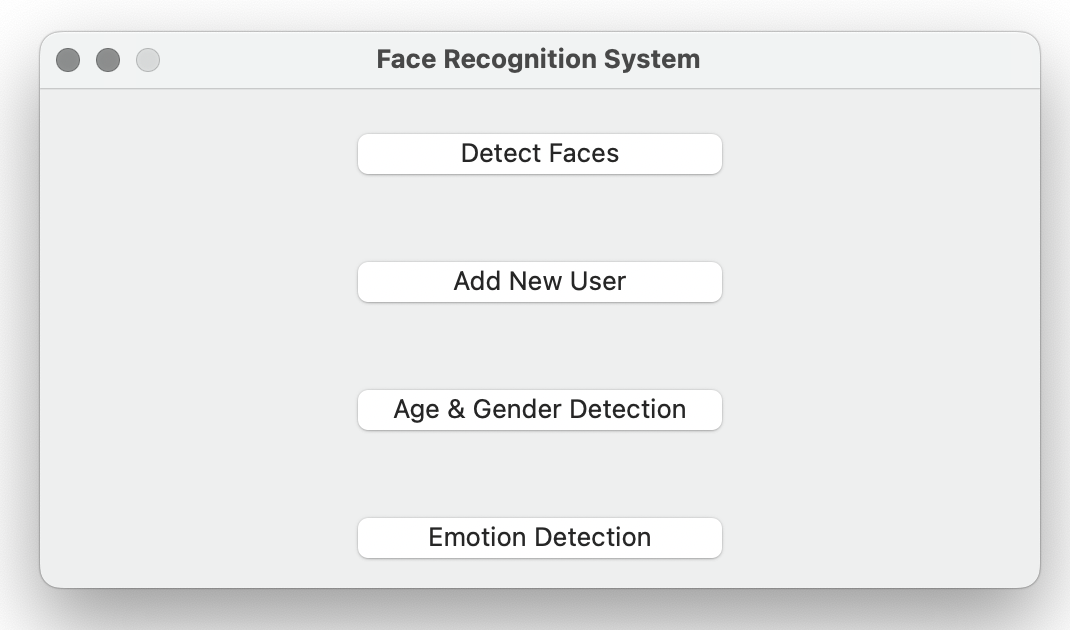
\includegraphics[width=0.7\textwidth]{capture1.png}
    \caption{Interface principale du système}
\end{figure}

\textbf{Interprétation} :  
Cette figure montre la fenêtre principale du logiciel. L'utilisateur peut ici capturer une image, lancer la reconnaissance faciale, ou entraîner le modèle avec de nouvelles données.

\vspace{0.5cm}

\begin{figure}[H]
    \centering
    \includegraphics[width=0.7\textwidth]{chemin/vers/ta/capture2.png}
    \caption{Détection d'un visage en temps réel}
\end{figure}

\textbf{Interprétation} :  
Sur cette capture, le système détecte un visage en direct via la webcam. Les informations de reconnaissance et d'analyse (émotion, âge, genre) sont affichées sur l'interface utilisateur.

\section{Tests Réalisés}

Différents tests ont été effectués pour valider le bon fonctionnement du système :

\begin{itemize}
    \item \textbf{Test de détection faciale} : Vérification que les visages sont détectés correctement dans diverses conditions d'éclairage et d'orientation.
    \item \textbf{Test de reconnaissance} : Validation de la capacité du modèle LBPH à reconnaître correctement les individus enregistrés dans la base de données.
    \item \textbf{Test de robustesse} : Présentation d'images altérées (expressions faciales différentes, port de lunettes) pour tester la tolérance du système aux variations.
    \item \textbf{Test de performance} : Mesure du temps de traitement moyen pour la détection et la reconnaissance, assurant une exécution en temps quasi-réel.
    \item \textbf{Test d'interface utilisateur} : Évaluation de l'ergonomie et de la simplicité d'utilisation de l'application.
\end{itemize}

Les résultats des tests indiquent que le système atteint un bon compromis entre précision, vitesse et robustesse dans l'environnement prévu.

\chapter{Conclusion et Perspectives}

\section{Bilan Personnel}

Ce projet m'a permis de renforcer considérablement ma confiance en mes capacités techniques et méthodologiques.  
En développant un système de reconnaissance faciale fonctionnel, j'ai acquis une meilleure assurance dans la gestion de projets complexes, en particulier dans la structuration des tâches, la résolution de problèmes techniques, et l'adaptation aux imprévus.

La mise en œuvre pratique de concepts avancés tels que l'Analyse en Composantes Principales (PCA) et l'utilisation de modèles d'apprentissage automatique m'a donné une vision concrète de l'application des théories étudiées en cours.

\section{Bilan Professionnel}

Sur le plan professionnel, ce projet a conforté mon intérêt pour le domaine de l'intelligence artificielle, du traitement d'images et de l'apprentissage automatique.  
Je souhaite désormais m'orienter vers une spécialisation en vision par ordinateur et en machine learning, domaines porteurs et en constante évolution.

Cette expérience m'a également sensibilisé à l'importance des considérations pratiques telles que l'efficacité des algorithmes, l'optimisation des temps de traitement, et la conception d'interfaces utilisateurs accessibles.

\section{Perspectives et Conclusion}

Le projet est globalement une réussite :  
le système développé atteint les objectifs fixés, à savoir la détection et la reconnaissance faciale en temps réel dans un environnement contrôlé, avec un bon compromis entre précision et rapidité.

Cependant, plusieurs axes d'amélioration peuvent être envisagés pour enrichir et rendre le système plus robuste :

\begin{itemize}
    \item Intégration de méthodes de deep learning plus avancées pour améliorer la précision de la reconnaissance faciale.
    \item Extension du système à des environnements non contrôlés (variations d'éclairage, arrière-plans complexes).
    \item Optimisation du temps de traitement pour permettre la reconnaissance en temps réel sur des dispositifs mobiles.
    \item Mise en place d'une base de données centralisée et sécurisée pour la gestion des utilisateurs.
\end{itemize}

En conclusion, ce projet constitue une première étape solide vers des réalisations plus ambitieuses en intelligence artificielle appliquée, et il ouvre la voie à de nombreuses perspectives d'évolution aussi bien académiques que professionnelles.



\chapter{Fonctionnalité Principale du Programme}
\begin{itemize}
    \item \textbf{Prétraitement des Images} : \textit{Préparation de dataset}.
    \begin{itemize}
        \item Détection et rognage des visages
        \item Conversion en niveaux de gris (0–255)
        \item Alignement des visages
        \item Réduction du bruit (application de filtres gaussiens ou médians)
    \end{itemize}

    \vspace{0.2cm}
    \begin{figure}[ht]
        \centering
        \scalebox{1}{%
            \begin{tabular}{*{7}{c}}
                
\includegraphics[height=1.2cm,keepaspectratio]{face_crop.jpg} & 
                \raisebox{0.5cm}{$\Rightarrow$} & 
                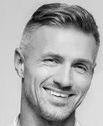
\includegraphics[height=1.2cm,keepaspectratio]{grayscale.jpg} & 
                \raisebox{0.5cm}{$\Rightarrow$} & 
                \includegraphics[height=1.2cm,keepaspectratio]{alignment.jpg} & 
                \raisebox{0.5cm}{$\Rightarrow$} & 
                \includegraphics[height=1.2cm,keepaspectratio]{denoise.jpg} \\
                \scriptsize\textbf{(1) Détection} & & 
                \scriptsize\textbf{(2) Conversion} & & 
                \scriptsize\textbf{(3) Alignement} & & 
                \scriptsize\textbf{(4) Débruitage} \\
            \end{tabular}%
        }
        \caption{Processus de prétraitement des images faciales}
        \label{fig:preprocessing_flow}
    \end{figure}
\end{itemize}

\begin{itemize}
    \item \textbf{Extraction des données avec ACP} : \textit{Préparation de dataset}.
    \begin{itemize}
        \item Calcul des Eigenfaces (les vecteurs propres associés)
        \item Réduction de dimensions (sélection des composantes principales)
        \item Optimisation du nombre de composantes
    \end{itemize}
\end{itemize}

%\begin{frame}{Conformité RGPD et Sécurité des Données}
    \begin{itemize}
        \item \textbf{Protection et gestion sécurisée des données faciales} :
        \begin{itemize}
            \item Conformité aux exigences du RGPD pour la collecte et le traitement des données personnelles.
            \item {Chiffrement des données sensibles} : Utilisation de l'algorithme AES-256 pour assurer la confidentialité et l'intégrité des données stockées.
            \item Mise en œuvre d’un accès restreint et d’une journalisation des accès afin d’assurer la traçabilité.
        \end{itemize}
        
    \end{itemize}

\chapter{Comparaison FaceID vs. Notre Système}
\begin{center}
\begin{tabular}{|p{3cm}|p{4cm}|p{4cm}|}
\hline
\textbf{Critère} & \textbf{FaceID (Apple)} & \textbf{Notre Système (ACP+SVM)} \\
\hline
Acquisition & TrueDepth (IR 3D) & Images 2D prétraitées \\
\hline
Méthode & Deep Learning + Liveness & ACP (Eigenfaces) + SVM \\
\hline
Sécurité & Secure Enclave local & Chiffrement AES-256, accès restreint \\
\hline
Robustesse & Très robuste (variations) & Conditions contrôlées \\
\hline
RGPD & Traitement local & Conformité via chiffrement \\
\hline
Matériel & Matériel dédié (IR, projecteur) & Caméras standards \\
\hline
Performance & Déverrouillage instantané & Dépend de l'optimisation \\
\hline
\end{tabular}
\end{center}


    \vspace{0.5cm}
%\begin{frame}{Estimation des Budgets}
    \begin{center}
    \begin{tabular}{|l|l|}
        \hline
        \textbf{Projet} & \textbf{Budget Estimé} \\
        \hline
        R\&D Apple Face ID & $\sim$1 milliard \$ (Not official) \\
        \hline
        Notre Projet & coffee+laptop+internet..:P \\
        \hline
    \end{tabular}
    \end{center}
    \vspace{0.5cm}

\chapter{Diagramme de GANTT}
\def\mystartdate{2025-03-17}
\def\myenddate{2025-04-04} % Shortened range for better fit

\centering % Center the following content
\scalebox{0.7}{ % Scale to fit inside Beamer slide
\begin{ganttchart}[
    today={2025-03-28},
    today rule/.style={draw=red!80, dash pattern=on 3.5pt off 4.5pt, line width=1.5pt},
    today label font=\bfseries\small,
    today label=Today,
    hgrid style/.style={draw=black!70, line width=.1pt},
    vgrid={*1{draw=black!30, line width=.1pt}},
    x unit=0.8cm, % Reduce width per day
    inline,
    title height=1,
    y unit title=5mm,
    milestone inline label node/.style={right=2cm}, 
    bar inline label node/.style={right=2cm}, % Adjusted label padding
    bar label font=\mdseries\color{black!70},
    bar label node/.append style={right=-3cm},
    bar/.append style={draw=none, fill=blue!60}, 
    bar incomplete/.append style={fill=blue!30}, 
    bar progress label font=\mdseries\footnotesize\color{black!70},
    group/.append style={fill=blue!40}, 
    group label node/.append style={left=.4cm},
    link/.style={-latex, thick, ->, red, rounded corners=1mm},
    milestone/.append style={fill=red, rounded corners=1pt},
    time slot format=isodate
]{\mystartdate}{\myenddate}

\gantttitlecalendar{week, weekday=letter, day} \\

\ganttbar{Réunion 1}{2025-03-20}{2025-03-20} \\
\ganttbar{Définition des fonctionnalités principales}{2025-03-20}{2025-03-22} \\
\ganttbar{Réunion 2}{2025-03-21}{2025-03-21} \\
\ganttbar{Recherche sur ACP}{2025-03-21}{2025-03-24} \\
\ganttbar{Étude de faisabilité}{2025-03-23}{2025-03-26} \\
\ganttbar{Étude comparative}{2025-03-24}{2025-03-27} \\
\ganttbar{Réunion 3}{2025-03-24}{2025-03-24} \\
\ganttbar{Réunion 4}{2025-03-28}{2025-03-28} \\
\ganttbar{Rédaction du rapport}{2025-03-20}{2025-03-29}
\end{ganttchart}
} % End of scalebox

\chapter{Détection des visages}
\begin{itemize}
    \item \textbf{Objectif :}  
          Identifier et localiser automatiquement les zones d'une image contenant des visages humains.
    \item \textbf{Principe de base :}  
          Il s'agit d'un problème de classification binaire : pour chaque sous-région (ou fenêtre) de l'image, la décision est « visage » ou « non-visage ».
\end{itemize}
\begin{figure}[ht]
    \centering
    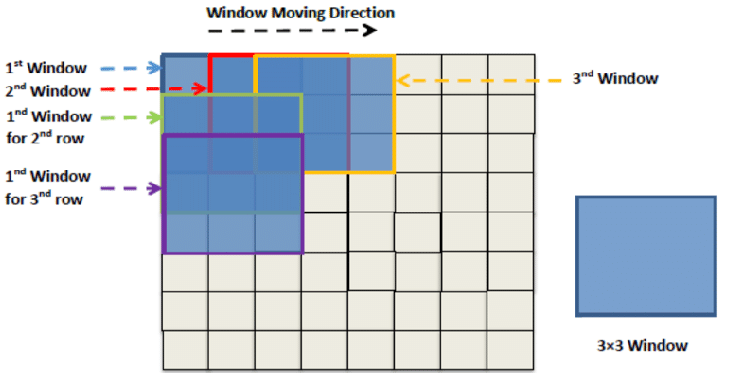
\includegraphics[width=0.6\textwidth]{sliding_window.png} % Remplacer par le nom de votre image
    \caption{Schéma illustrant la détection des visages par classification binaire}
    \label{fig:face_detection}
\end{figure}

\chapter{Petite Intro à l'ACP}
\textbf{Analyse en Composantes Principales (ACP)} est une technique statistique utilisée pour :
\begin{itemize}
    \item Réduire la dimensionnalité des données tout en conservant l'essentiel de l'information.
    \item Identifier les directions principales de variation des données.
    \item Faciliter la visualisation et l'interprétation des structures complexes.
\end{itemize}

\textbf{Principe :} Trouver de nouvelles variables (composantes principales) qui sont des combinaisons linéaires des variables d'origine et qui maximisent la variance.

\textbf{Applications :}
\begin{itemize}
    \item Compression et réduction de bruit.
    \item Visualisation de données en haute dimension.
    \item Prétraitement pour l'apprentissage automatique.
\end{itemize}

\textbf{Algorithme de calcul}
\footnotesize
\begin{enumerate}
    \item \textbf{Centrage des données} \\
    Soit $X\in\mathbb{R}^{n\times p}$, avec :
    \begin{itemize}
        \item $\mu_j=\frac{1}{n}\sum_{i=1}^{n}x_{ij}$, pour $j=1,\dots,p$,
        \item $X'=X-\mathbf{1}\mu$, avec $\mathbf{1}$ le vecteur colonne de 1.
    \end{itemize}
    \item \textbf{Matrice de covariance} \\
    \[
    C=\frac{1}{n-1}(X')^T X'
    \]
    \item \textbf{Valeurs et vecteurs propres} \\
    Résoudre :
    \[
    C\,v=\lambda\,v.
    \]
    \item \textbf{Tri} \\
    Ordonner les $\lambda_1\ge\lambda_2\ge\cdots\ge\lambda_p$ et conserver les vecteurs propres correspondants.
    \item \textbf{Projection} \\
    Choisir $k$ vecteurs pour former $V_k\in\mathbb{R}^{p\times k}$ et projeter :
    \[
    Z=X'\,V_k.
    \]
\end{enumerate}

\chapter{Conception et Modélisation (UML)}
\begin{figure}[h]
\centering
\scalebox{1}{ % Scale down the entire diagram
\begin{sequencediagram}
    \newinst{user}{Utilisateur}
    \newinst[0.5]{ui}{UI} % Reduced spacing between instances
    \newinst[0.5]{attendance}{AttendanceSystem}
    \newinst[1]{eigen}{EigenfacesSystem}
    \newinst[1]{proc}{ImageProcessor}
    \newinst[0.5]{pca}{PCA}
    \newinst[0.5]{svm}{SVM}
    
    \begin{call}{user}{\footnotesize Lance l'attendance}{ui}{}
    \end{call}
    
    \begin{call}{ui}{\footnotesize mark\_attendance()}{attendance}{}
        \begin{call}{attendance}{\footnotesize recognize()}{eigen}{}
            \begin{callself}{eigen}{\footnotesize Traitement Eigenfaces}{}
                \begin{call}{eigen}{\footnotesize capture\_image()}{proc}{}
                    \begin{callself}{proc}{\footnotesize preprocess()}{}
                    \end{callself}
                \end{call}
                
                \begin{call}{eigen}{\footnotesize project(face)}{pca}{\footnotesize coefficients[m]}
                \end{call}
                
                \begin{call}{eigen}{\footnotesize predict(coefficients)}{svm}{\footnotesize student\_id}
                \end{call}
            \end{callself}
        \end{call}
    \end{call}
    
    \begin{call}{attendance}{\footnotesize Affiche résultat}{ui}{}
    \end{call}
\end{sequencediagram}
}
\caption{\footnotesize Diagramme de séquence Eigenfaces Recognition}
\label{fig:eigenfaces_seq}
\end{figure}

\chapter{Bibliographies et Webographie}
\begin{thebibliography}{9}

\bibitem{bts_doc}
Principal Component Analysis (PCA) – \textit{GeeksForGeeks} Website. 
\href{https://www.geeksforgeeks.org/principal-component-analysis-pca/}{[Lien]} 

\bibitem{cal_doc}
Face Detection using Haar Cascades – \textit{OpenCV}. 
\href{https://docs.opencv.org/3.0-beta/doc/py_tutorials/py_objdetect/py_face_detection/py_face_detection.html}{[Lien]} 

\bibitem{labri_doc}
"Robust Real-Time Face Detection" (PDF). – \textit{Archived from the original (PDF)} on 2019-02-02.
\href{https://web.archive.org/web/20190202042433/http://www.vision.caltech.edu/html-files/EE148-2005-Spring/pprs/viola04ijcv.pdf}{[Lien]} 

\bibitem{wikidoc11}
Viola–Jones object detection framework – \textit{Wikipedia}.
\href{https://en.wikipedia.org/wiki/Viola–Jones_object_detection_framework}{[Lien]} 

\bibitem{karim_nolink}
karimnolink – \textit{test 1} (lien non disponible).
\alert{[Lien non disponible]}

\end{thebibliography}
\end{document}